\documentclass[11pt, english]{article}\usepackage[]{graphicx}\usepackage[]{color}
%% maxwidth is the original width if it is less than linewidth
%% otherwise use linewidth (to make sure the graphics do not exceed the margin)
\makeatletter
\def\maxwidth{ %
  \ifdim\Gin@nat@width>\linewidth
    \linewidth
  \else
    \Gin@nat@width
  \fi
}
\makeatother

\definecolor{fgcolor}{rgb}{0.345, 0.345, 0.345}
\newcommand{\hlnum}[1]{\textcolor[rgb]{0.686,0.059,0.569}{#1}}%
\newcommand{\hlstr}[1]{\textcolor[rgb]{0.192,0.494,0.8}{#1}}%
\newcommand{\hlcom}[1]{\textcolor[rgb]{0.678,0.584,0.686}{\textit{#1}}}%
\newcommand{\hlopt}[1]{\textcolor[rgb]{0,0,0}{#1}}%
\newcommand{\hlstd}[1]{\textcolor[rgb]{0.345,0.345,0.345}{#1}}%
\newcommand{\hlkwa}[1]{\textcolor[rgb]{0.161,0.373,0.58}{\textbf{#1}}}%
\newcommand{\hlkwb}[1]{\textcolor[rgb]{0.69,0.353,0.396}{#1}}%
\newcommand{\hlkwc}[1]{\textcolor[rgb]{0.333,0.667,0.333}{#1}}%
\newcommand{\hlkwd}[1]{\textcolor[rgb]{0.737,0.353,0.396}{\textbf{#1}}}%
\let\hlipl\hlkwb

\usepackage{framed}
\makeatletter
\newenvironment{kframe}{%
 \def\at@end@of@kframe{}%
 \ifinner\ifhmode%
  \def\at@end@of@kframe{\end{minipage}}%
  \begin{minipage}{\columnwidth}%
 \fi\fi%
 \def\FrameCommand##1{\hskip\@totalleftmargin \hskip-\fboxsep
 \colorbox{shadecolor}{##1}\hskip-\fboxsep
     % There is no \\@totalrightmargin, so:
     \hskip-\linewidth \hskip-\@totalleftmargin \hskip\columnwidth}%
 \MakeFramed {\advance\hsize-\width
   \@totalleftmargin\z@ \linewidth\hsize
   \@setminipage}}%
 {\par\unskip\endMakeFramed%
 \at@end@of@kframe}
\makeatother

\definecolor{shadecolor}{rgb}{.97, .97, .97}
\definecolor{messagecolor}{rgb}{0, 0, 0}
\definecolor{warningcolor}{rgb}{1, 0, 1}
\definecolor{errorcolor}{rgb}{1, 0, 0}
\newenvironment{knitrout}{}{} % an empty environment to be redefined in TeX

\usepackage{alltt}
\usepackage{amsmath,amssymb,latexsym}

%\usepackage{palatino}
%\usepackage{arev}
\usepackage{fourier}
%\usepackage{antpolt}

\usepackage{graphicx}
\usepackage{tikz-qtree}
\usepackage{amscd}
\usepackage{bbm}
\usepackage{caption}
\usepackage[utf8]{inputenc}
\usepackage[T1]{fontenc}
\usepackage{babel}
\usepackage{rotating,amssymb,amsmath,amsfonts,delarray}
\usepackage{geometry}
\usepackage{placeins}
\usepackage{caption}
\usepackage{float}
\usepackage{amsthm}
\newtheorem*{remark}{Remark}
\geometry{hmargin=80pt, vmargin=70pt}
\usepackage{amsfonts}
\usepackage{xcolor}
\usepackage{hyperref}
\usepackage{enumerate}
\usepackage{enumitem}
\usepackage{tikz}
\usepackage{cancel}
\usepackage{scalerel,stackengine}

\usepackage{forest}

\colorlet{mygreen}{green!75!black}
\colorlet{col1in}{red!30}
\colorlet{col1out}{red!40}
\colorlet{col2in}{mygreen!40}
\colorlet{col2out}{mygreen!50}
\colorlet{col3in}{blue!30}
\colorlet{col3out}{blue!40}
\colorlet{col4in}{mygreen!20}
\colorlet{col4out}{mygreen!30}
\colorlet{col5in}{blue!10}
\colorlet{col5out}{blue!20}
\colorlet{col6in}{blue!20}
\colorlet{col6out}{blue!30}
\colorlet{col7out}{orange}
\colorlet{col7in}{orange!50}
\colorlet{col8out}{orange!40}
\colorlet{col8in}{orange!20}
\colorlet{linecol}{blue!60}

\hypersetup{
  colorlinks=true,
  citecolor=blue,
  linkcolor=blue,
  filecolor=magenta,
  urlcolor=cyan,
}

\newtheorem{rem}{Remark}
\newtheorem{deff}{Definition}
\newtheorem{lem}{Lemma}
\newtheorem{ex}{Example}
\newtheorem{theorem}{Theorem}
\newtheorem{algo}{Algorithm}

\setlength{\parindent}{0cm}

\setlength\parindent{0pt}

\title{The \texttt{nCopula} package}
\author{David Beauchemin \\ Simon-Pierre Gadoury}
\date{\today}
\IfFileExists{upquote.sty}{\usepackage{upquote}}{}
\begin{document}

\maketitle

\begin{abstract}
The \emph{nCopula} package aims to simplify the construction process and usage of hiearchical Archimedean copulas through compound distributions in \texttt{R}. Is is possible to build structures with clear representations, obtain expressions for Archimedean copulas, wether they are hiearchical or not, as well as other important functions (i.e. Laplace Stieltjes Transform, pgf, etc.), given a certain path and structure. Furthermore, the generation of random vectors is possible from any given structure.
\end{abstract}

\section{Introduction}

Let us consider different situations to illustrate how one can use the various functions in the package \texttt{nCopula}.

\section{Generating vectors from defined structures}

\begin{figure}[!h]
  \centering
  \begin{tabular}{cccc}
    \textbf{Node} & \textbf{Distribution} & \textbf{Parameter} & \textbf{Dimension} \\
    \hline
    $M^{(0)}$ & Geometric & $0.5$ & 3 \\
    $M^{(0,1)}$ & Geometric & $0.1$ & 2 \\
    $\Theta^{(0,1,1)}$ & Gamma & $0.1$ & 2 \\
    $\Theta^{(0,1,2)}$ & Gamma & $0.2$ & 2 \\
    $\Theta^{(0,2)}$ & Gamma & $0.01$ & 2 \\
    $M^{(0,3)}$ & Geometric & $0.5$ & 2 \\
    $\Theta^{(0,3,1)}$ & Geometric & $0.01$ & 2\\
    $\Theta^{(0,3,1)}$ & Logarithmic & $0.9$ & 2\\
    \hline
  \end{tabular}
\end{figure}

\begin{figure}[H]
\centering
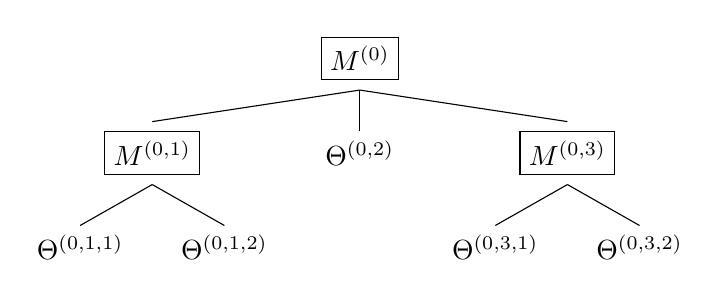
\begin{tikzpicture}[scale=1, level distance=12mm, sibling distance=5mm]
  \Tree [.\fbox{$M^{(0)}$} [.\fbox{$M^{(0,1)}$} $\Theta^{(0,1,1)}$ $\Theta^{(0,1,2)}$ ] $\Theta^{(0,2)}$ [.\fbox{$M^{(0,3)}$} $\Theta^{(0,3,1)}$ $\Theta^{(0,3,2)}$ ] ]
\end{tikzpicture}
\caption{}
\end{figure}

\newpage

\bibliographystyle{apalike}
\bibliography{BibRRT}

\end{document}
